
%%%%%%%%%%%%%%%%%%%%%%%%%%%%%%%% 
\section{The Time Projection Chamber (TPC)} 
\label{sec:detectors-fd-ref-tpc}

\subsection{Overview}

The scope of the Time Projection Chamber (TPC) subsystem includes the
design, procurement, fabrication, testing and delivery of anode plane
assemblies (APAs), cathode plane assemblies (CPAs), the field cage and
the high voltage system.

The TPC is an active detector element of each DUNE
far detector module. It is located inside the cryostat vessel and is
completely submerged in liquid argon at 88~K. 
%The TPC consists of
%alternating anode plane assemblies (APAs) and cathode plane assemblies
%(CPAs), with field-cage modules enclosing the four open sides between
%the anode and cathode planes.  
The TPC is constructed of modular elements called
 anode plane assemblies (APAs),  cathode plane assemblies
(CPAs), and field-cage modules. The APAs and CPAs are assemblies of
wire planes, and they are tiled into alternating APA-CPA rows along the length of
the cryostat. The resulting rows are called \textit{anode planes} and \textit{cathode planes}, respectively.
(Note the different uses of the word \textit{plane}.)  Field-cage modules enclose the four open sides between
the anode and cathode planes.  
%
When proper bias voltages are applied
to the APAs and CPAs, a uniform electric field is created in the volume
between the anode and cathode planes. A charged particle traversing
this volume leaves a trail of ionization in the ultra-pure liquid
argon.  The electrons drift toward the anode wire planes, inducing
electric current signals in the front-end electronic circuits
connected to the sensing wires.  The current-signal waveforms from all
sensing wires are amplified and digitized by the front-end electronics
and transmitted through cold (immersed) cables and feedthroughs to the data
acquisition (DAQ) system outside of the cryostat. While electrons drift
toward the APAs, positive ions drift toward the CPAs at a velocity five orders of 
magnitude slower than that of the electrons and therefore contribute little to the signal on the wires.  



\begin{cdrfigure}[Cross section of the TPC inside the cryostat]{tpc-xsect1}
{Cross sections of the LBNE \ktadj{5} TPC (left) and the DUNE \ktadj{10} TPC (right).  
The exchange of the APA and CPA positions significantly reduces the energy 
stored in the TPC by eliminating the two ground-facing cathode planes. 
This allows an increase in the detector's fiducial volume given the same cryostat volume. %with the same cryostat.  
The length of the DUNE TPC is  58~m along the direction of the neutrino beam (into the page).}
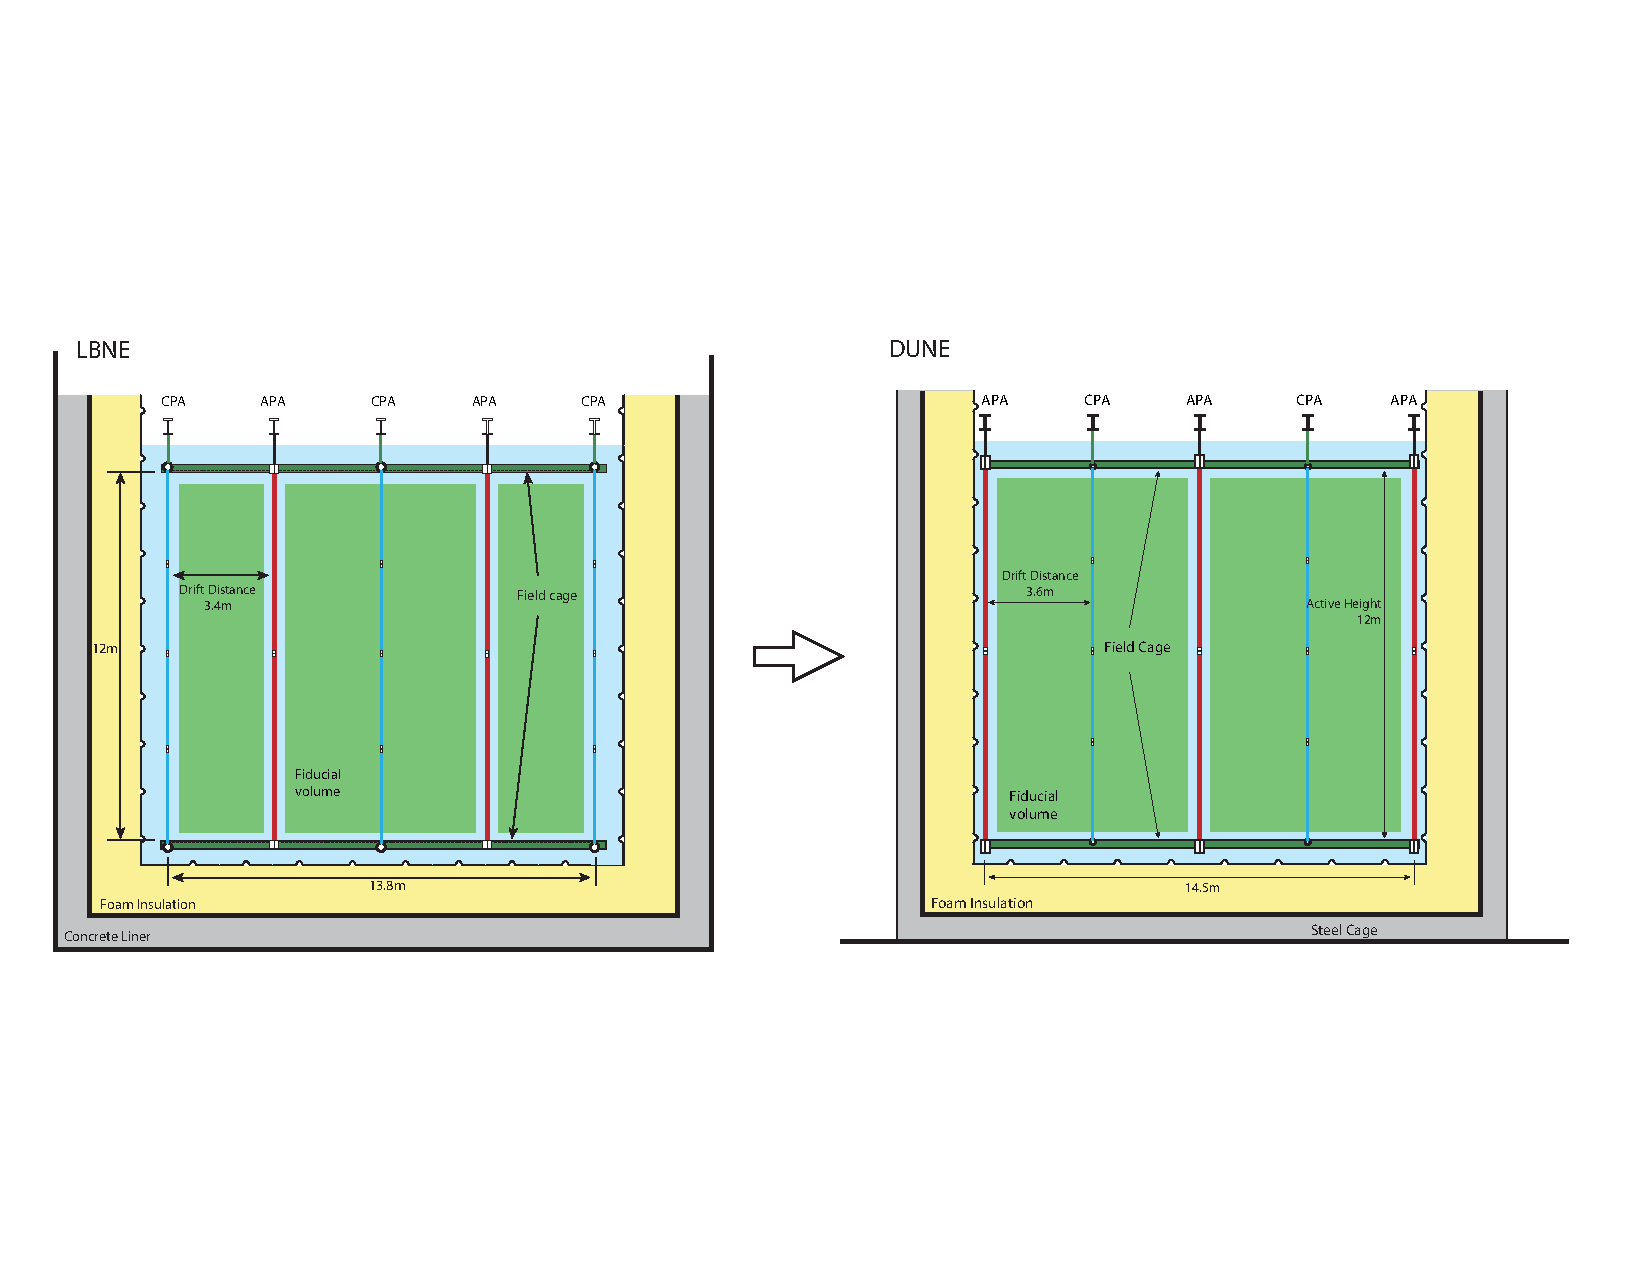
\includegraphics[width=\linewidth]{tpc_xsection_lbne_dune.pdf}
\end{cdrfigure}
The TPC active volume (Figure~\ref{fig:tpc-xsect1}) is 12~m high,
14.5~m wide and 58~m long in the beam direction.  
Its three rows of APA planes interleaved with two rows of CPA planes
are oriented vertically, with the planes parallel to the beamline. The
electric field is applied perpendicular to the planes.  The maximum
electron-drift distance between a cathode and an adjacent anode is
3.6~m. This requires a $-$180~kV bias voltage on the cathode plane to
reach the 500~V/cm nominal drift field. The anode plane assemblies are
2.3~m wide and 6~m high. Two 6~m modules are stacked vertically to
instrument the 12~m active depth. In each row, 25 such stacks are
placed edge-to-edge along the beam direction, forming the 58~m active
length of the detector.  Each CPA has the same width, but half the
height ($\sim$3~m) as an APA, for ease of assembly and transportation.
Four CPAs will be stacked vertically to form the full 12-m active
height.  Each cryostat houses a total of 150~APAs and 200~CPAs.  Each
facing pair of cathode and anode rows is surrounded by a field
cage assembled from panels of FR-4 glass-reinforced epoxy laminate
sheets with parallel copper strips connected to resistive divider
networks.  The entire TPC is suspended from five mounting rails under the
cryostat ceiling (see Figure~\ref{fig:tpc-floor-view}).

\begin{cdrfigure}[A view of the partial assembled TPC]{tpc-floor-view}
{A view of the partially installed TPC inside the membrane cryostat.
  The APAs are shown in red, CPAs are in cyan, field-cage modules in
  yellow/green.  Some of the field-cage modules are in their folded
  position against the cathode (providing aisle access during installation).}
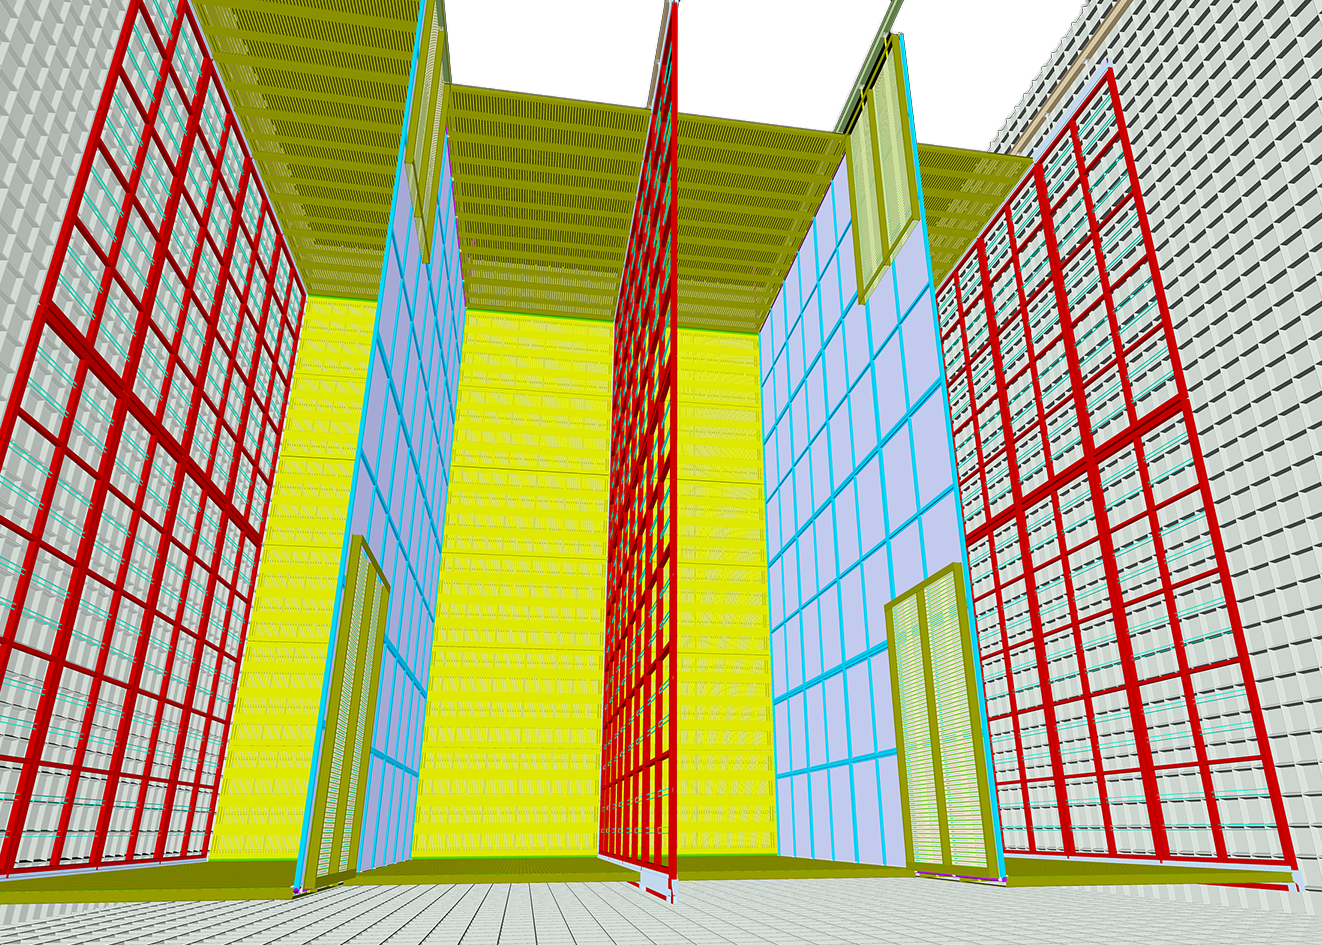
\includegraphics[width=\linewidth]{tpc_floor_view.png}
\end{cdrfigure}

The units of construction of the active detector are the APAs, CPAs,
and field-cage modules. These are modular elements of a size optimized
so as to simplify the manufacture, satisfy the commercial highway and
underground transport requirements, and facilitate the handling and 
%speedy 
efficient installation in the cryostat.  
APAs and CPAs 
Each element will be fully
tested in LN$_2$ (or LAr) at the assembly site, again at the far
detector site before installation, and finally will be monitored
continuously during and after installation to detect any failures.

%%%%%%%%%%%%%%%%%%%%%%%%%%%%%%%% 
\subsection{Anode Plane Assemblies (APA)}
\label{subsec:fd-ref-apa}

An APA is constructed from a framework of
lightweight, rectangular stainless steel tubing, with four layers of
wires wrapped on each side of the frame.
% added sentence about the wires -- it's more important than the dimensions of the thing
From the outside in, the first wire layer is a shielding (grid) plane, next are
two induction planes and the collection plane. 
%
The front-end electronics
boards are mounted on one end of the APA
frame and protected by a
metal enclosure.
The APAs are 2.3~m wide, 6.3~m high, and 12~cm thick. The height is
chosen for fabrication purposes and compatibility with underground
transport limitations. The 2.3-m width is set to fit in a standard
HiCube container \fixme{hicube.com or hicubecoating.com? or something else?}
for storage and transport with sufficient shock
absorbers and clearances.  


%%%%%%%%%%%%%%%%  
\subsubsection{Wire Planes}
\label{subsec:fd-ref-wireplanes}

Wire of 150~$\mu$m diameter copper beryllium (CuBe) alloy is used on the
APAs for high tensile strength, good electrical conductivity,
excellent solderability and a thermal-expansion coefficient
compatible with that of the stainless steel frame.  The wires will be
epoxied to fiberglass wire-bonding boards and then soldered to copper
traces on the boards for electrical connections.

Four planes of wires cover each side of an APA frame as shown in Figure~\ref{fig:tpc-wire-frame-xsect}.

\begin{cdrfigure}[Illustration of the APA wire wrapping scheme]{tpc-wire-frame-xsect}{Illustration of the APA wire wrapping scheme (left), and three cross sectional views (right). At left, small portions of the wires from the three signal planes are
shown in color: magenta (U), green (V), blue (X). The fourth wire
plane  (G) above these three, parallel with X, is present to improve the pulse shape
on the U plane signals. At right, the placement of the wire planes relative to the stainless steel frame is shown for different locations
on the APA. See Table~\ref{wire-parameters} for wire plane parameters.}
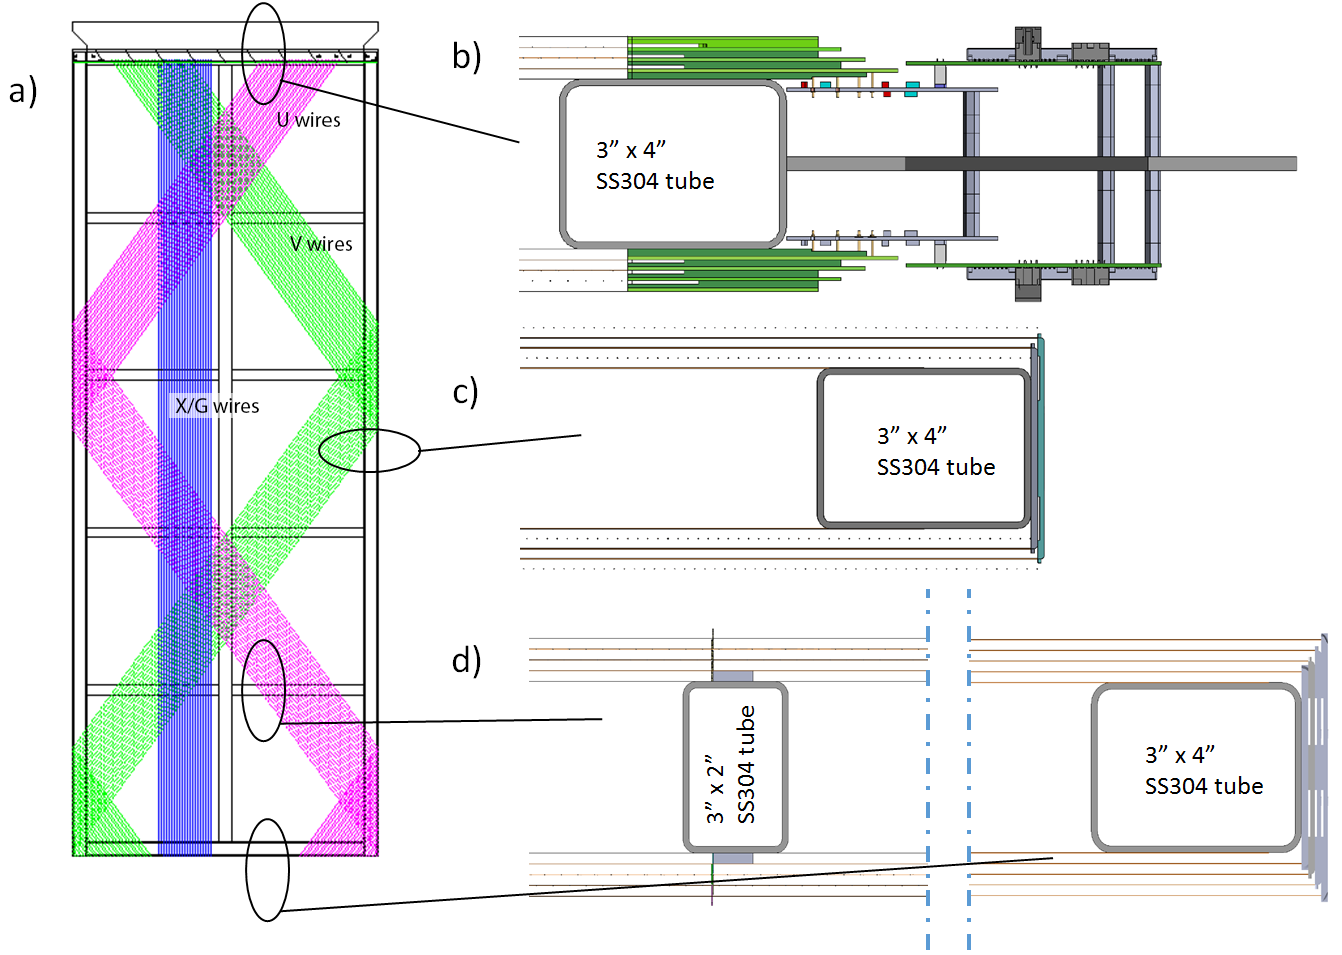
\includegraphics[width=0.8\linewidth]{tpc_apa_cross_sections}
\end{cdrfigure}
These four planes of wires are labeled, in order from the outside in:
G (for grid), U, V and X.  Table~\ref{tab:wire-parameters} summarizes
the key parameters of each of the wire planes.  
\begin{cdrtable}[Wire parameters]
  {llrrrr}{wire-parameters} {Parameters of the four planes of wires on an APA}
  
   Label & Function & Orientation &  Pitch & Number  & Bias Voltage 		\\ \rowtitlestyle
      			&						& (from vertical) 		& {(mm)}   	&   			& {(volt)} 	\\ \colhline
    G    		& Shield/grid plane 			&0$^\circ$  			& 4.79		& 960 		& $-$655   \\ \colhline
    U            	&  1$^{st}$ induction plane 	& +35.7$^\circ$  		& 4.67		&  800  		& $-$365 	\\ \colhline
    V            	&  2$^{nd}$ induction plane	& $-$35.7$^\circ$  	& 4.67	 	&  800  		& 0 			\\ \colhline
    X            	&  Collection plane			& 0$^\circ$ 			& 4.79 		&  960  		& +860 		\\

\end{cdrtable}
The distance between wire planes is 4.76~mm (3/16 inch, a standard printed
circuit board thickness).  Each wire plane is biased to a particular
voltage such that the ionization electrons from charged particle
tracks will drift past the first three wire planes and be completely
collected by the %last 
collection wire plane (X).  The V wires are DC-coupled to
the readout electronics to minimize the maximum voltage on the other
wire planes.  A grounded mesh plane with good optical transparency,
located 4.8~mm behind the collection plane, prevents the electric
field around this set of wires from being distorted by the metal frame
structure and the wires on the opposite side of the frame. It also
shields the sensing wires from potential EM interference from the
silicon photomultipliers (SiPMs) on the photon detectors, mounted
within the frame.  Each wire on the U, V and X planes is connected to a
front-end readout channel. The grid plane wires are not read out, but
serve the important purpose of shielding the U wires from responding
to distant moving charges. The total number of readout channels in an
APA is 2560, for a total of 384,000 in each cryostat.

The wires on the two induction planes (U and V) are wrapped in a
helical pattern around the long edges of the wire frame
(Figure~\ref{fig:tpc-wire-frame-xsect}a). This technique makes it
possible to place readout electronics only at one short edge of an APA
frame, and allows tiling of the APAs on the other three sides with
minimal dead space ($\sim$1.3\% of active area).  Although wires on the %both 
induction planes are sensitive to tracks on both sides of an APA,
the vertical collection-plane wires are only sensitive to one side, and
therefore able to resolve this ambiguity.  The upper APAs in the
cryostat will have their readouts at the top edge of the frame (as
shown in Figure~\ref{fig:tpc-wire-frame-xsect}), while the lower APAs
will mount their electronics at the bottom edge.  These readout
electronics are located within the LAr volume but \fixme{check edit here} outside of the TPC active volume.  On the
readout end of an APA, 20 sets of front-end readout boards with 128
channels each (40U+40V+48X) are distributed on both sides of the APA,
reading out the \SI{2560} sense wires.

With the APA length and width constrained by transportation and handling
limitations, the angles on the induction plane wires are chosen so
that they wrap less than one full revolution around the APA.  This
avoids an ambiguity problem where three wires from three readout
planes intersect more than once on an APA face (discussed in 
Section~\ref{v4:fd-ref-wireangle}).  Precise values of
wire angle and wire pitch (see Table~\ref{tab:wire-parameters}) were
chosen to give an integral number of wires across the boards at the
electronics end of the APA as well as an integral number of wire slots
in the boards along the sides of the APA.  A preliminary
study\cite{wire-orientation} has shown that this wire layout meets the
physics requirements.

The APAs facing the cryostat walls are sensitive on both sides, similar to
 those in the middle of the TPC.  However, the negative bias
voltage on their outer grid planes prevents any electrons drifting
from the cryostat walls toward the sensing wires.  The electronics for
the outer X wire plane can be eliminated to save cost.  Alternatively, %we can utilize 
these double-sided APAs can be utilized by adding another cathode plane
with a small negative bias between the cryostat wall and the anode plane to
form a very shallow veto region.

%%%%%%%%%%%%%%%%
\subsubsection{APA Frame}
\label{subsec:fd-ref-apaframes}

At the nominal wire tension of 5~N, the total of \SI{3520} wires exerts a
force of $\sim$7.0~kN/m on the short edges of the APA, and a
$\sim$1.5~kN/m force on the long edges. The wire frame must be able to
withstand the wire tension with minimal distortion, while minimizing
the thickness of the frame to reduce the resulting dead space. \fixme{resulting from what?} The
wire frame is constructed from stainless steel tubes welded in a
jig.  Structural analysis has shown that the maximum distortion of the
frame due to wire tension is less than 0.5~mm. The total mass of a
bare frame is $\sim$260~kg.

%% Lengthwise buckling is not an issue, both because of the strength of the frame and because the wires are maintained at an approximately uniform distance from the frame by periodic comb-like structures.

All tube sections are vented to prevent the creation of trapped
volumes. \fixme{of LAr?} The three long tubes have slots cut in them so the photon
detectors can be inserted into the APAs after the wires are installed. \fixme{this is important because...}
The two long outer members of the frame are open-ended, so the photon
detector cables can be threaded through them to reach the signal
feedthroughs on the cryostat roof.  These long tubes can potentially
be used to carry signal and power cables from the bottom APAs' cold
electronics boards to the signal feedthroughs, as well.  This could significantly 
reduce the cable length %for these APAs 
compared to, e.g.,
running the cables from the middle bottom APAs % charge readout cables on 
along the floor and then up the wall.


%%%%%%%%%%%%%%%%
\subsubsection{APA Wire Bonding and Support}
\label{subsec:fd-ref-wirewrap}


The wire bonding boards physically anchor the wires at the edges of an
APA and provide the interface between the wires and the cold
electronics at the readout end of the APA.  The four planes of wires
are attached to their respective wire bonding boards through a
combination of epoxy and solder. During winding of the X layer onto
the APA, the wires are placed across the top surface of the X wire
board. The wires are then glued down with a strip of epoxy at the
leading edge of the board.  After the epoxy has cured, the wires are
soldered onto the copper pads under each wire, and then the wires are
cut beyond the pads. The V, U and G planes are attached on top of the
X boards and similarly populated with wires, one layer at a time. An
array of pins is pushed through holes in the stack of wire bonding
boards, making electrical connections between the wires and the
capacitor-resistor (or CR) board, which is located between the wire
boards and the front-end electronics boards.  The CR boards distribute
the bias voltages to each wire through current-limiting 20~M$\Omega$
resistors, and bring the charge signal through high voltage AC
coupling capacitors to the cold electronics.

These readout boards, as described in
Section~\ref{sec:detectors-fd-ref-ce}, generate an estimated
$\sim$160~W of heat per APA which may produce a small quantity of
argon bubbles.  Stainless steel covers are placed over the readout
boards to contain the bubbles and direct them to the gas volume of the
cryostat. This is particularly important for the bottom APAs where the
bubbles must be contained and funneled through the vertical hollow
frame members to the top of the cryostat to prevent the bubbles
entering the TPC active volume.

Comb-like wire support structures (see Figure~2.9 in \anxlbnefd) are
located on each of the four cross beams (see Figure~\ref{fig:tpc-wire-frame-xsect})
 so that the longitudinal wires
are supported every 1.2~m and the angled wires about every 1.5~m while
introducing only millimeter-scale dead regions. The support structure
is composed of strips of thin G10 sheet, with notches machined at
correct intervals.  These wire supports play a key role in minimizing
wire deflection due to gravity and electrostatic force, enabling the
use of a moderate wire tension and reducing the risk of wire breakage.
They also maintain the correct wire pitch and wire plane separation
even if the APA frame has a small amount of twist and warp.  If a wire
breaks after installation, these intermediate wire support will limit
the movement of the broken wire such that it will not travel too far
into the drift volume and make contact with the field cage.  To
further reduce the risk and impact of a broken wire, a new wire
support scheme is being developed that can be applied to the outer
wire planes near the bottom of the TPC to prevent a broken wire from
contacting the field cage.


%%%%%%%%%%%%%%%%
\subsubsection{Wire-winding Machines}
\label{subsec:fd-ref-wirewinding}

A winding machine will be constructed to lay the \SI{3520} wires onto each
APA. It has sufficient versatility that the same mechanism can wind
both the angled and the longitudinal layers.
 
Its working concepts are illustrated in
Figure~\ref{fig:tpc-winding-machine}.
\begin{cdrfigure}[Winding machine concepts]{tpc-winding-machine}
{Illustration of the wire winding machine concept.  The tensioner 
head is passed from one side of the APA to the other as it is moved 
around the APA to wind wire onto the APA frame.  The horizontal/vertical 
positioning systems on each side of the APA are made of commercial linear motion components. }
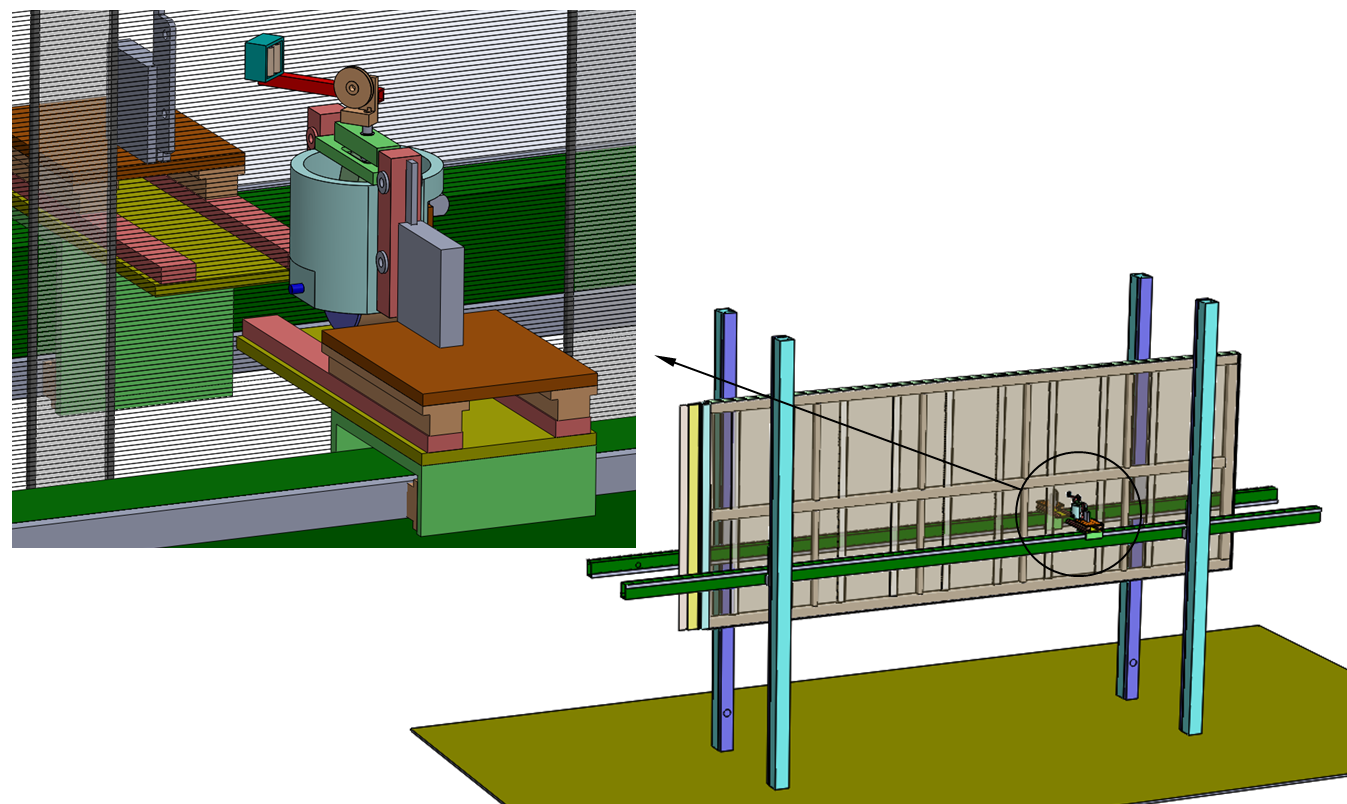
\includegraphics[width=0.9\linewidth]{tpc_apa_winding_machine.png}
\end{cdrfigure}
The wire tensioner is a self-contained unit that includes the wire
spool.  It is designed so that correct wire tension is maintained,
independent of the wire-feed rate and direction.  The APA,
oriented horizontally in the device (with one of its long edges down), is held off
the ground by a couple of posts.  \fixme{check edit} There
are X-Y positioners on either side of the APA; the tensioner is moved
across the face of the APA by one of these positioners, unspooling
tensioned wire as it moves.  When the tensioner arrives at the edge of
the APA it is passed across to the positioner on the other side of the APA
while placing the wire into the appropriate slots of the edge
boards. \fixme{at the edge of the board?} In this way the entire layer of wire can be placed on the
frame. 

Although a large part of an entire plane of wires can be wound in one
continuous process, a more fault-tolerant procedure will be adopted in which %would be to pause
the winding machine will be paused periodically to solder the last wire \fixme{winding?}. This
intermediate soldering step will prevent the unraveling of a large
section due to an accidental broken wire.  An automatic soldering
robot will solder the wire ends after the wires have been laid down on
the APA. A wire-tension measuring device will scan the newly placed
wires and record the wire tension of each wire. Any wires with
abnormal tension will be replaced manually.


%%%%%%%%%%%%%%%%%%%%%%%%%%%%%%%%
\subsection{Cathode Plane Assemblies (CPAs)}
\label{subsec:fd-ref-cpa}

There are two cathode planes in each detector module.  Each cathode plane is 
tiled from a four-unit-high by 25-unit-wide array of CPAs. Figure~\ref{fig:tpc-cathode-model} shows the
building blocks of a cathode plane.  
\begin{cdrfigure}[Conceptual design of cathode plane components ] 
{tpc-cathode-model}{Conceptual design of the cathode plane 
components near a corner.  Two flavors of CPAs (outer 
and inner unit) are used to make up the entire cathode plane; all
CPAs are roughly 2.3~m wide by 3~m tall. 
The cathode plane is terminated at %both 
right and left ends by the end pieces (cyan colored).  An HV receptacle 
(orange) connects with the HV feedthrough from the cryostat ceiling. }
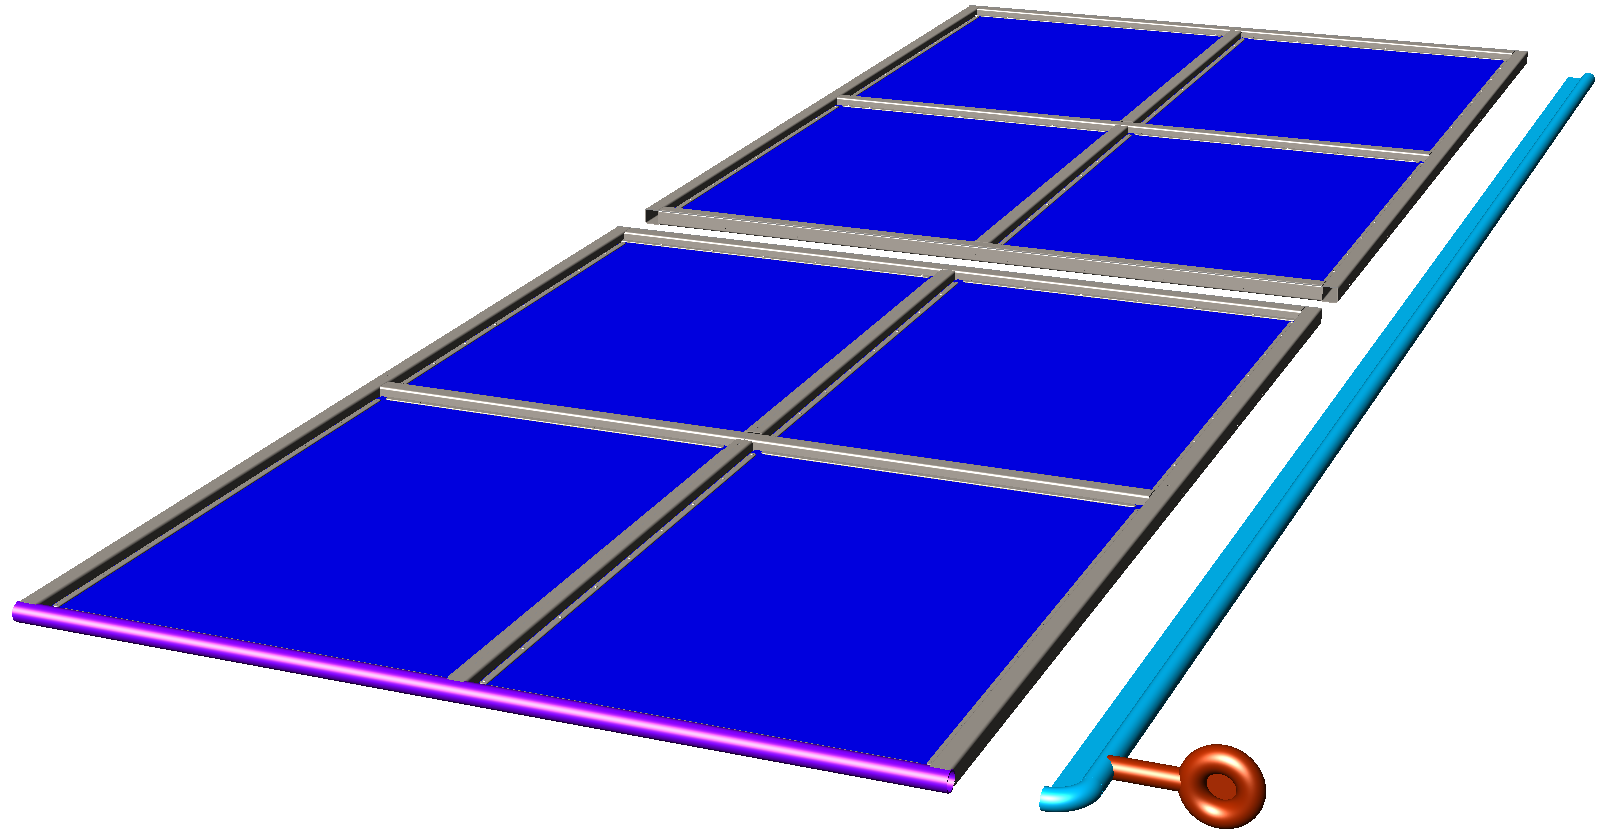
\includegraphics[width=0.9\linewidth]{tpc_cpa_components}
\end{cdrfigure}

Each CPA is 2.3~m wide (identical to the APA width) and 3~m tall (half
of APA height) for ease of fabrication, assembly and handling.  Each
CPA is made of a stainless steel framework, with panels of solid
stainless steel sheets mounted between the frame openings.  Along each
vertical column of %the 
four CPAs, there are two slightly different
versions: the outer CPAs (top and bottom rows ), and the inner CPAs
(2$^{nd}$ and 3$^{rd}$ rows).  The inner CPAs use all rectangular tubes for the
frame structure, while the outer CPAs use 5~cm OD round tubes on the
outside edge of the CPA facing the floor or ceiling of the cryostat to
minimize the surface electric field \fixme{magenta in Figure~\ref{fig:tpc-cathode-model} ?}.  Two sets of field-shaping end
pieces are installed at the two ends (e.g., right and left) of a CPA wall to properly
terminate the cathode wall with rounded edges.  All CPAs are suspended
from the ceiling using G10 hangers under fiberglass rails to insulate
the CPAs from the cryostat.

A recent design decision exchanged the positions of the CPAs and APAs
in the detector relative to the earlier LBNE reference design, placing the APAs adjacent to the cryostat wall
instead of the CPAs. % as in the LBNE reference design.  
This change
reduces the stored energy on each cathode plane by about 60\%.
Nevertheless, due to the enormous area of the stainless steel cathode
plane, there is still nearly 100~Joules of energy when biased at
180~kV, risking physical damage to the thin membrane structure as well
as to the CPA structure in the event of a high voltage discharge.  In
addition, in such an event, a huge voltage swing could occur on the
cathode plane in tens of nanoseconds, injecting a charge pulse to the
sensing wires with a large peak current that could damage the
front-end electronics.

To mitigate this risk, analysis of the electrical properties of the
cathode has been carried out with the goal of developing a cathode
design that will substantially slow down the total energy release in
case of a discharge.  The best solution appears to be replacing the
metallic cathode structure by non-conductive materials with a robust
and highly resistive surface coating.  Many choices of 
resistive/anti-static coating and commercially produced
anti-static sheet materials are available.  Studies are underway to identify a
suitable coating and base material for this application.  Since the
electrical current feeding the field cage resistive dividers is
supplied through the cathode, a special current-distribution feature
must be designed to minimize voltage drop along this 58-m-long, highly
resistive structure.


%%%%%%%%%%%%%%%%%%%%%%%%%%%%%%%%
\subsection{Field Cage}
\label{subsec:fd-ref-fieldcage}

In the TPC, each pair of facing cathode and anode planes forms an
electron-drift region. A field cage must completely surround the four
open sides of this region to provide the necessary boundary conditions
to ensure a uniform electric field within, unaffected by the presence
of the cryostat walls.


Each \ktadj{10} detector module requires $\sim$2000~m$^2$ of field
cage coverage. In the current reference design, the field cages are
constructed using multiple copper-clad FR-4 sheets reinforced with
fiber glass I-beams to form modules of 2.3~m $\times$ 3.6~m in
size. Parallel copper strips are etched on the FR-4 sheets using
standard printed circuit board fabrication techniques. Strips are
biased at appropriate voltages provided by a resistive-divider \fixme{resistor-divider?}
network. These strips create a linear electric-potential gradient in
the LAr, ensuring a uniform drift field in the TPC active volume. \fixme{or in the drift volume? At least the direction
will differ in different drift volumes}
Simulations have shown that the non-uniformity of the drift field quickly
drops to about 1\%, roughly a strip pitch away from the field-cage
surface.

Since the field cage completely encloses the TPC drift region on four
sides, while the solid cathodes block the remaining two, the field
cage sheets must be perforated to allow LAr recirculation in
the middle third of the TPC volume. The ``transparency'' of the
perforation will be determined by a detailed LAr computerized fluid
dynamic (CFD) study.

The resistor-divider network will be soldered directly onto the
field-cage panels. Multiple resistors will be connected in parallel
between any two taps of the divider, in order to provide fault
tolerance. 
\fixme{`taps' not defined; maybe readers will know, but I don't}
One end of the divider chain is connected directly to the
cathode, while the other end is connected to ground at the APA through
resistors of the appropriate value.  %It is envisioned that 
A pair of
field-cage modules will likely be %are 
pre-attached to the outer CPA modules through
hinges, %and 
such that the field-cage modules can be rotated into their final
position during installation, or folded back if aisle access is needed
(see Figure~\ref{fig:tpc-floor-view}).  In addition to the resistor-divider
network, surge suppressors such as varistors or gas discharge tubes
will be installed between the field-cage strips to avoid the occurrence of an
over-voltage condition between field-cage electrodes and the
cathode in the event of a high voltage discharge.

The major challenge of this field-cage design is 
minimizing exposure of the electric field to the LAr
%electric field exposed to the LAr 
near the thin copper
strips.  One solution is to cover all copper edges with a thick layer
of solder mask (an acrylic-based polymer with a high dielectric
strength) as part of the standard PCB fabrication process.  This
construction is currently being implemented in the 35-t prototype TPC (see
Sec~7.5 of \anxlbnefd).  Figure~\ref{fig:tpc-field-cage} shows a
section of this partially constructed field cage.  
\begin{cdrfigure}[35-t field cage]{tpc-field-cage}{A corner of the 35-t TPC 
field cage during construction}
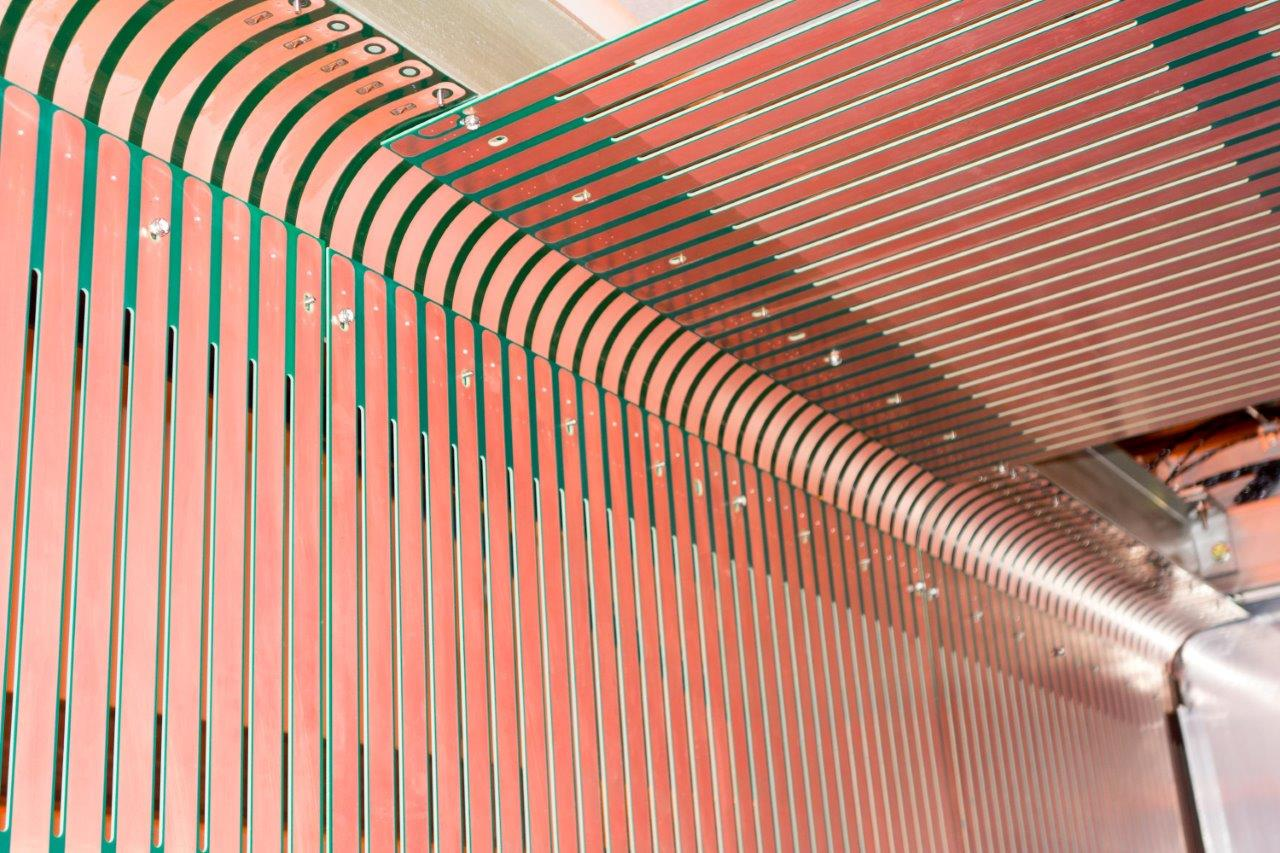
\includegraphics[width=4in]{tpc_fca_35t.jpg}
\end{cdrfigure}
The 35-t prototype test results will be evaluated to determine if this
technique is suitable for the much larger far detector modules.
 
In the meantime, alternative concepts are being actively developed to
further minimize the electric field on the field cage.  One example is application of %to apply 
a very high resistive \fixme{high-resistance} coating on the outside surface of the
field cage such that the surface potential distributes uniformly
across the gaps between conductors and therefore eliminates the high-field
region near the conductor edges.  The challenge here is %how to
ventilation of this field cage surface without significantly increasing the
field at the edge of the perforations.  Another concept is to use
roll-formed metal profiles as the field-cage electrodes supported by \fixme{and support them using}
insulating beams.  These profiles have large edge radii; this makes
their surface electric field relatively low, which in turn makes it possible
to place them %be placed 
even closer to the cryostat walls to improve the
efficiency of LAr use.  %One particular 
A sample profile is shown in
Figure~\ref{fig:tpc-field-cage-roll-form}.  
\begin{cdrfigure}[FCA with roll-formed metal profile]{tpc-field-cage-roll-form}
{Left: electrostatic simulation of a field cage design that uses roll-formed 
metal profiles as the field-cage electrodes.  Right: a conceptual design of a 
field-cage module using this profile.}
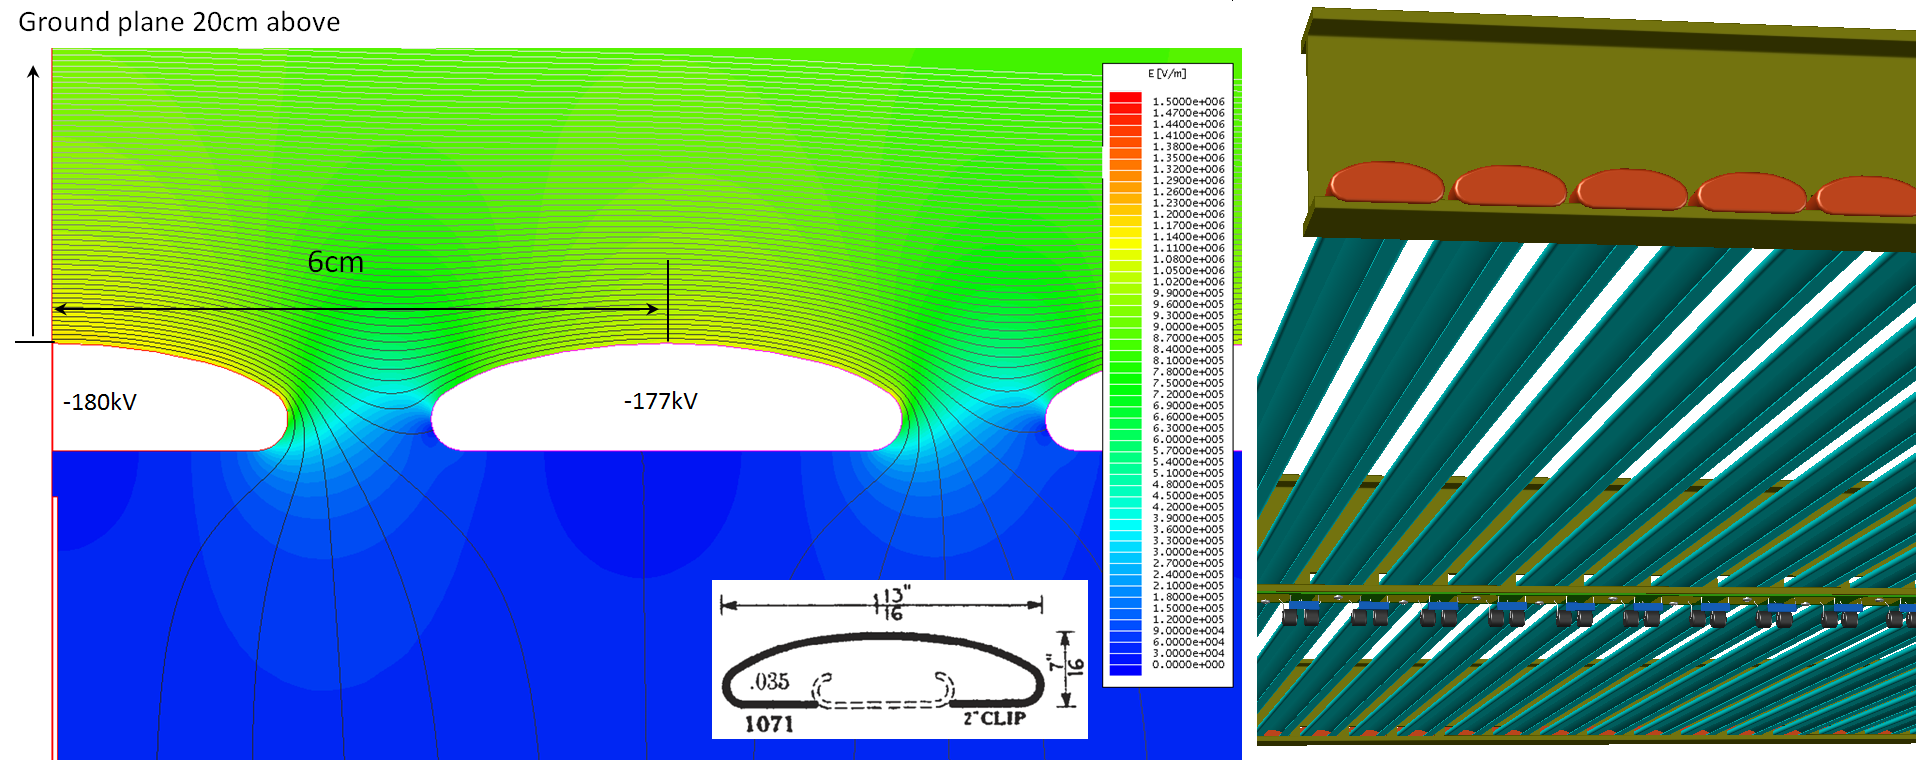
\includegraphics[width=\linewidth]{tpc_fca_rollform.png}
\end{cdrfigure}
With only a 20-cm distance %away 
separating the field cage from a ground plane, the electric field on the field cage is
still under 12~kV/cm.  The ends of the profiles still have high
electric field, however; a possible solution is to cover the ends with UHMW
polyethylene caps.  This design may also cost significantly less than
the reference design with PCBs.


%%%%%%%%%%%%%%%%%%%%%%%%%%%%%%%%
\subsection{High Voltage Components}  
\label{subsec:fd-ref-hv}
   
The two cathode planes are biased at $-$180~kV to provide the required
500~V/cm drift field. Each cathode plane will be powered by a
dedicated HV power supply through an RC filter and feedthrough.

The power supplies for the cathode planes must be able to provide
$-$200~kV at 1~mA current. The output voltage ripple must not
introduce more than 10\% of the equivalent thermal noise from the
front-end electronics.  The power supplies must be programmable to
trip (shutdown) their output at a certain current limit.  During power
on and off, including output loss (for any reason), the voltage ramp
rate at the feedthrough must be controllable to prevent damage to the
in-vessel electronics %through 
from excess charge injection.  High-voltage
feedthroughs must be able to withstand $-$250~kV at their center
conductors in 1~atm argon gas environment when terminated in liquid
argon.


The current candidate for the high-voltage power supplies is the
Heinzinger PNC{\it hp} series, which has the lowest output ripple
specification.  Additional filtering of the voltage ripples is done
through the intrinsic HV cable capacitance and series resistors
installed inside the filter box. Established techniques and practices
will be implemented to eliminate micro-discharges and minimize
unwanted energy transfer in case of an HV breakdown.
  
To ensure safe and reliable operation, the feedthroughs will be tested
at a much higher voltage than expected in routine operation
($\sim$250~kV) in LAr. The feedthroughs will be mounted on
the ceiling of the cryostat, their cold ends reaching through the gas
ullage space and submerging into the LAr. The center
conductor on the cold side of a feedthrough will be insulated and
shielded by a grounded shroud at least 50~cm below the surface of the
liquid to ensure bubble free operation at the
tip. Figure~\ref{fig:tpc-UCLA-feedthrough} shows an example of the
feedthrough and filter box made by the UCLA group for the 35-t prototype TPC,
as well as the conceptual design of a feedthrough suitable for the far
detector TPCs.
\begin{cdrfigure}[Concept of new feedthrough]{tpc-UCLA-feedthrough}
{Top: The high voltage feedthrough and filter developed by the UCLA 
group for the 35-t TPC.  It was tested up to 150~kV.  
Bottom: a conceptual design of a new feedthrough for the far detector.}
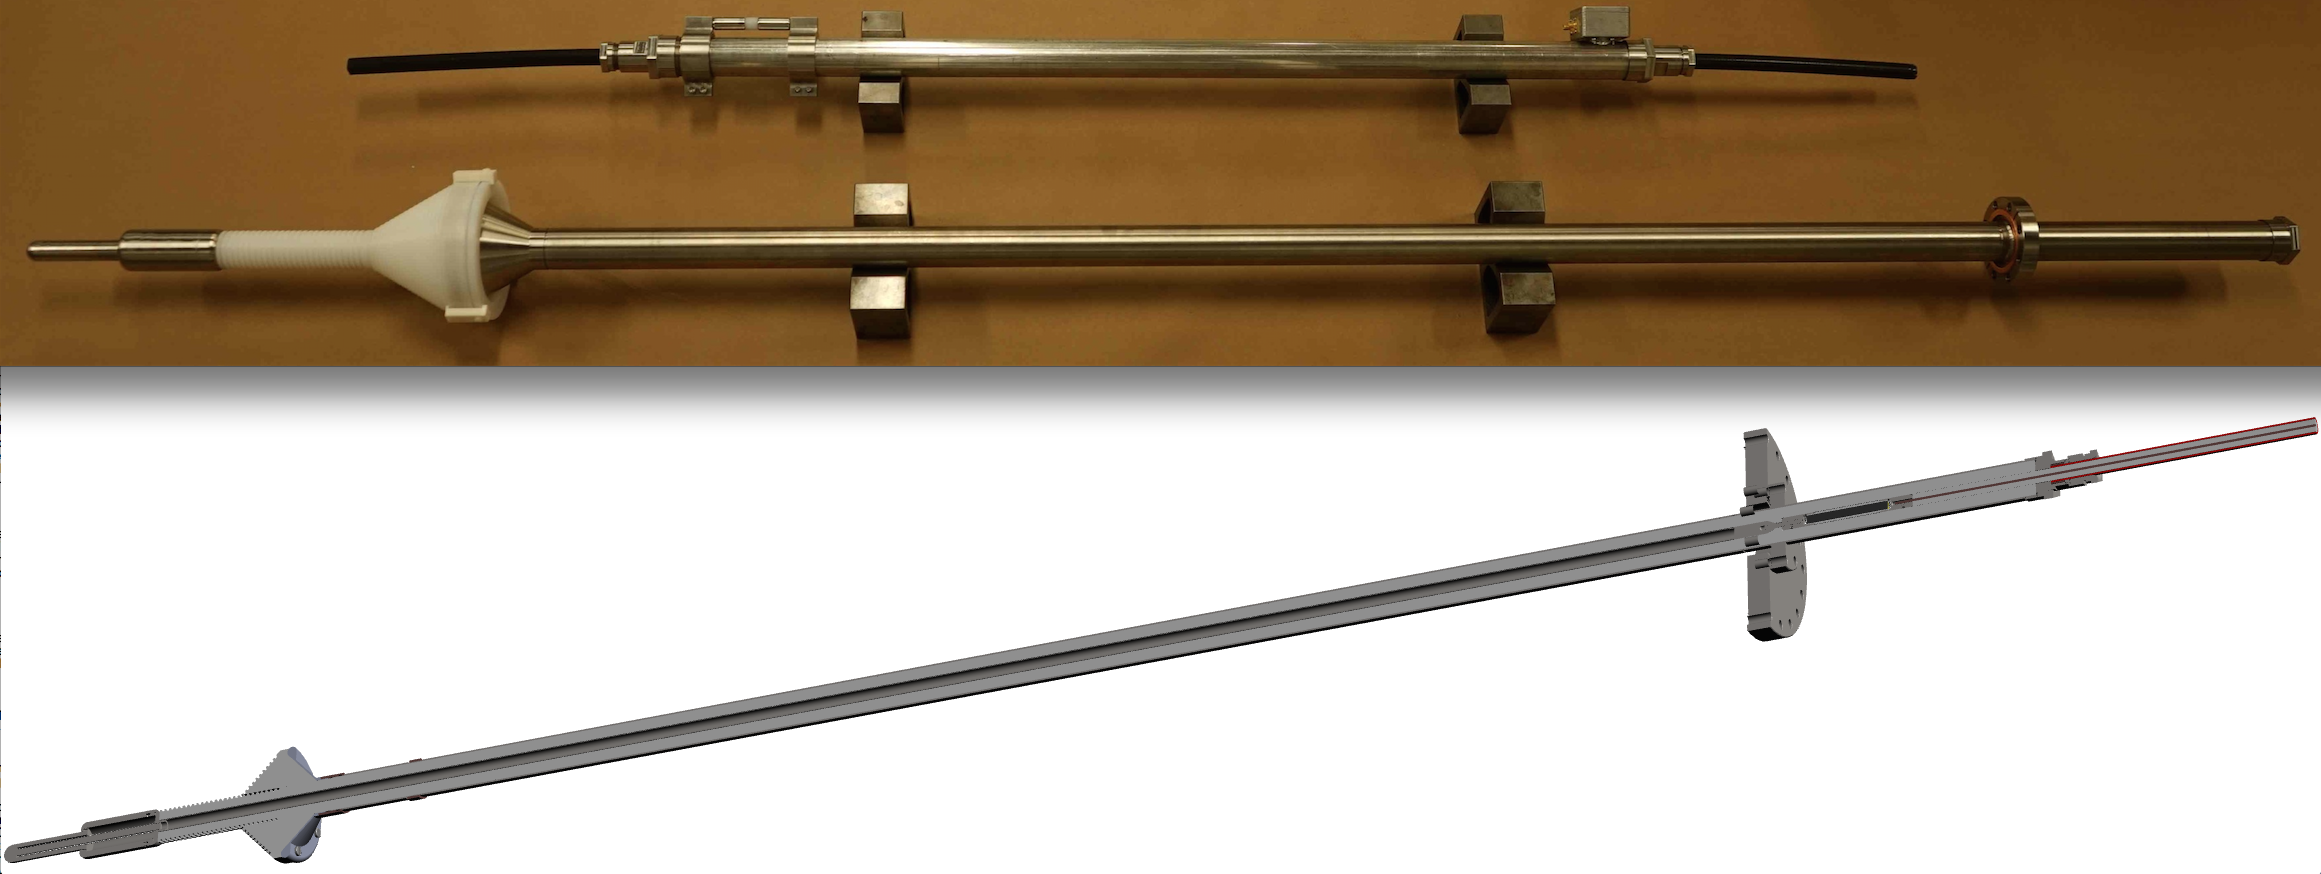
\includegraphics[width=\linewidth]{tpc_hv_feedthrough.png}
\end{cdrfigure}

\fixme{Would be nice to give dimensions in caption to figure \ref{tpc-UCLA-feedthrough}}


%%%%%%%%%%%%%%%%%%%%%%%%%%%%%%%%
\subsection{TPC Prototyping and Tests}
\label{subsec:fd-ref-tpc-proto}


Several prototype TPC modules were constructed during the design phase
of the LBNE project. The initial prototypes were fractional-scale
or partial models of the APA and CPA. The CPA prototype was used to
evaluate field-shaping electrode attachment techniques. A 40\% scale
APA prototype was constructed earlier on to study the placement of the
wire-wrapping boards and wire-support structures. It was also used to
develop the prototype winding machines. The prototypes were subjected
to numerous thermal cycles down to liquid-nitrogen temperature to test
the integrity of the wire-to-board and board-to-frame bonds.

\fixme{Started out with `they WERE made back in LBNE days.' Now this next one is current?}
The second set of prototypes are scale models of the APA and CPA. They
are being used to validate the designs and to evaluate production
procedures. These functional prototypes will be installed in the 35-t
prototype cryostat  %This TPC is 
and are expected to be operational in 2015.

A TPC prototype proposed for installation %to go into 
in a CERN test beamline
requires six full-size APAs with fully instrumented readout electronics,
six full-size CPAs and complete field cage coverage. This prototype will be %The TPC will be
constructed using identical APAs, CPAs and field-cage panels as
designed for the far detector. Additional features will be installed
to ensure proper TPC operation given the half-height cryostat
configuration. The construction and assembly of all TPC mechanical
components will use the same materials and techniques as designed for
the far detector, with the exception of the degree of automation for wiring
the APAs, which will be reduced.

%a reduced degree of automation
%than will be used to wire APAs.
